%%% LaTeX Template: Two column article
%%%
%%% Source: http://www.howtotex.com/
%%% Feel free to distribute this template, but please keep to referal to http://www.howtotex.com/ here.
%%% Date: February 2011

%%% Preamble
\documentclass[	DIV=calc,%
paper=a4,%
fontsize=12pt,%
onecolumn]{scrartcl}	 					% KOMA-article class

\usepackage{lipsum}													% Package to create dummy text
\usepackage[brazil]{babel}										% English language/hyphenation
\usepackage[protrusion=true,expansion=true]{microtype}				% Better typography
\usepackage{amsmath,amsfonts,amsthm}					% Math packages
\usepackage[pdftex]{graphicx}									% Enable pdflatex
\usepackage[svgnames]{xcolor}									% Enabling colors by their 'svgnames'
\usepackage[hang, small,labelfont=bf,up,textfont=it,up]{caption}	% Custom captions under/above floats
\usepackage{epstopdf}												% Converts .eps to .pdf
\usepackage{subfig}													% Subfigures
\usepackage{booktabs}												% Nicer tables
\usepackage{fix-cm}													% Custom fontsizes
\usepackage[utf8]{inputenc}
\usepackage[top=2.5cm, bottom=2.5cm, left=2.5cm, right=2.5cm]{geometry}
\usepackage[ddmmyyyy]{datetime}
\addto\captionsenglish{%
	\renewcommand\tablename{Tabela}
	\renewcommand\figurename{Figura}
} 



%%% Custom sectioning (sectsty package)
\usepackage{sectsty}													% Custom sectioning (see below)
\allsectionsfont{%															% Change font of al section commands
	\usefont{OT1}{phv}{b}{n}%										% bch-b-n: CharterBT-Bold font
}

\sectionfont{%																% Change font of \section command
	\usefont{OT1}{phv}{b}{n}%										% bch-b-n: CharterBT-Bold font
}



%%% Headers and footers
\usepackage{fancyhdr}												% Needed to define custom headers/footers
\pagestyle{fancy}														% Enabling the custom headers/footers
\usepackage{lastpage}	

% Header (empty)
\lhead{}
\chead{}
\rhead{}
% Footer (you may change this to your own needs)

%% ====================================
%% ====================================
%% mude o rodape  do projeto
%% ====================================
%% ====================================

\lfoot{\footnotesize \texttt{Cabeamento estruturado} \textbullet ~Modelo de projeto}


\cfoot{}
\rfoot{\footnotesize página \thepage\ de \pageref{LastPage}}	% "Page 1 of 2"
\renewcommand{\headrulewidth}{0.0pt}
\renewcommand{\footrulewidth}{0.4pt}



%%% Creating an initial of the very first character of the content
\usepackage{lettrine}
\newcommand{\initial}[1]{%
	\lettrine[lines=3,lhang=0.3,nindent=0em]{
		\color{DarkGoldenrod}
		{\textsf{#1}}}{}}



%%% Title, author and date metadata
\usepackage{titling}															% For custom titles

\newcommand{\HorRule}{\color{DarkGoldenrod}%			% Creating a horizontal rule
	\rule{\linewidth}{1pt}%
}

\pretitle{\vspace{-30pt} \begin{flushleft} \HorRule 
		\fontsize{50}{50} \usefont{OT1}{phv}{b}{n} \color{DarkRed} \selectfont 
	}
	
	%% ====================================
	%% ====================================
	%% mude o titulo  do projeto
	%% ====================================
	%% ====================================
	
	\title{Projeto cabeamento estruturado Empresa}					% Title of your article goes here
	
	%% ====================================
	
	
	
	\posttitle{\par\end{flushleft}\vskip 0.5em}

\preauthor{\begin{flushleft}
		\large \lineskip 0.5em \usefont{OT1}{phv}{b}{sl} \color{DarkRed}}
	\author{Gelso Magdiel Gomes Baltazar}  	% Author name goes here
	
	
	\postauthor{\footnotesize \usefont{OT1}{phv}{m}{sl} \color{Black} 
		\\Minha Empresa								% Institution of author
		\par\end{flushleft}\HorRule}

\date{}																				% No date




%%% Begin document
\begin{document}
	\maketitle
	\thispagestyle{fancy} 	
	\thispagestyle{empty}		% Enabling the custom headers/footers for the first page 
	% The first character should be within \initial{}
	
	
	
	
	%% ====================================
	%% ====================================
	%% mude o resumo  do projeto
	%% ====================================
	%% ====================================
	\initial{E}\textbf{ste projeto tem por objetivo documentar a estrutura física existente, descrevendo sua topologia, analisando falhas, e propondo melhorias e soluções para o melhor funcionamento da rede.}
	
	%% ====================================
	\begin{figure}
		\centering
		\includegraphics{utfpr}
	\end{figure}
	
	\vspace{3cm}
	\centerline{\textit{\textbf{\today}}}
	
	\clearpage
	\renewcommand*\listfigurename{Lista de figuras}
	\listoffigures
	
	\renewcommand*\listtablename{Lista de tabelas}
	\listoftables
	
	
	
	
	\clearpage
	\renewcommand{\contentsname}{Sumário}
	\tableofcontents
	\clearpage
	
	%% ====================================
	%% ====================================
	%% Inicio do texto
	%% ====================================
	%% ====================================
	\section{Introdução}
	
	O presente documento será baseado em um provedor de internet. Atualmente a empresa possui 6 funcionários.
		O presente projeto tem por objetivo documentar a estrutura física de cabeamento na empresa para que possa trazer maior segurança aos técnicos que necessitarem realizar manutenções.
		O principal objetivo é documentar o estado atual do rack onde os dispositivos estão alocados e solucionar problemas encontrados por falta de documentação.		
	
	
	\subsection{Benefícios}
		\begin{itemize}
		\item Facilidade e agilidade na manutenção
		\item Claro entendimento de cada cabo e sua respectiva conexão
		\item Maior segurança e confiança para realizar manutenções
		\end{itemize}
	
	\subsection{Organizações Envolvidas}
		\begin{tabular}{|l|l|}
			\hline
			\textbf{Organização}                 & \textbf{Responsabilidade}                                                                                                                                          \\ \hline
			Organização 01                       & \begin{tabular}[c]{@{}l@{}}Cabeamento elétrico:\\ - Organizar cabeamento de rede elétrico\\ - Identificar cabeamento no rack e sua respectiva conexão\end{tabular} \\ \hline
			\multicolumn{1}{|c|}{Organização 02} & \begin{tabular}[c]{@{}l@{}}Cabeamento óptico:\\ - Organizar cabeamento ótico\\ - Identificar cabeamento no rack e sua respectiva conexão\end{tabular}              \\ \hline
		\end{tabular}
	
	
	
	\section{Estado atual}
	Atualmente a rede está instalada com cabeamento ótico e elétrico. Os equipamentos estão acomodados em um rack de piso 44U 19". No momento, por motivo de reestruração do cabeamento óptico, alguns cabos não estão acomodados corretamente até o término da manutenção.
	\begin{itemize}
		\item Passivos de rede: 
			\item  - patch panel
			\item  - cabo de rede CAT5
			\item  - patch cord CAT5
			\item  - cabo de rede CAT6
			\item  - patch cord CAT6
			\item  - cabo fibra óptica 36 FO
			\item  - cabo fibra óptica 12 FO
			\item  - DIO
			\item  - patch cord fibra óptica SC/UPC
			\item  - patch cord fibra óptica SC/APC
			
		\item as maiores reclamações dos usuários em relação ao cabeamento é a falta de documentação da mesma, pois isso causa insegurança na manutenção.Por esse motivo é necessário realizar a documentação do mesmo e reestruturar o cabeamento óptico para melhor acomodá-los aos DIO's.
		
	\end{itemize}
	
	\section{Requisitos}
	\begin{itemize}
		\item Reorganizar cabeamento
		\item Reorganizar equipamentos no rack
		\item Manter disponibilidade dos serviços
		\item Identificar cabeamento óptico e elétrico
	\end{itemize}
	
	\section{Usuários e Aplicativos}
	Atualmente os usuários utilizam aplicações web e mobile para interagir com o sistema. São sistemas que não demandam uso excessivo de banda na rede. Existem pontos de rede preparados para novas instalações em caso de contratação de novos funcionários.
	
	
	\subsection{Usuários}
	\begin{itemize}
		\item 06 funcionários;
		\item usuários de sistema web e mobile;
	\end{itemize}
	
	\subsection{Aplicativos}
	\begin{itemize}
		\item sistema web;
		\item sistema mobile;
		\item Sistemas utilizados para receber pagamentos e abrir chamados de usuários;
	\end{itemize}
	

	\section{Planta Lógica - Elementos estruturados}
	
	\subsection{Estado atual}
	Deve ter a planta atual, se for o caso
	
	\section{Estrutura predial existente}
	\begin{figure}
		\centering
		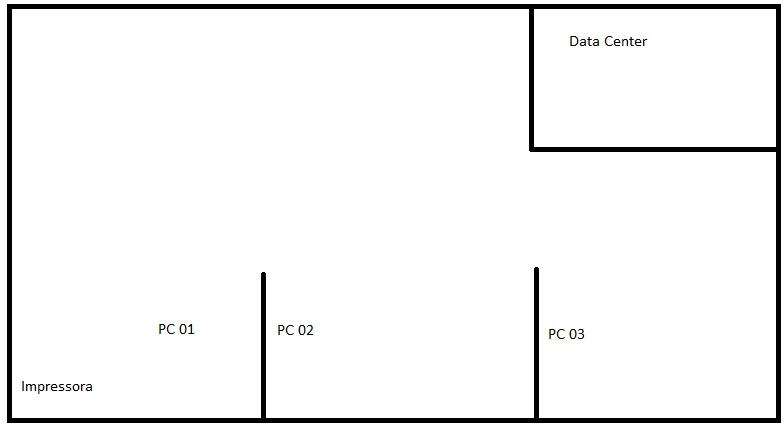
\includegraphics[width=\textwidth]{planta}
		\caption{Planta do prédio}
		\label{planta}
	\end{figure}
	
	Conforme a figura acima, pode-se ver que em cada divisória há um computador instalado e uma impressora de rede na mesma sala do PC 01.
	Os pontos de rede estão instalados na parede. Cada computador possui seu ponto de rede.
	Cada ponto de rede tem aproximadamente 10 metros de cabo até a sala do datacenter, onde há um patch panel que faz a ligação desse cabeamento com o switch. Os cabos estão passando por dentro de tubulação até a sala do datacenter.
	
	\subsection{Topologia}
	Após a implantação do cabeamento, a topologia da rede deverá estar como mostrado na figura 2. Os cabos da operadora irão chegar até o datacenter via fibra óptica subterrânea e deverá ser colocado em um DIO (Distribuidor Interno Óptico) para distribuição das fibras dentro do rack. 
	Do roteador sairá um cabo de rede CAT6 com conectores blindados que será conectado à uma OLT(Optical Line Termination) que fornecerá internet à clientes via fibra óptica.
	Do roteador sairá outro cabo de rede CAT6 com conectores blindados que estará interligado com o switch para rede interna. O switch estará conectado em um patch panel que fará a conexão com os computadores dentro da estrutura do prédio, conforme demonstrado na figra 1.
	
	%\input{tab1}
	\begin{figure}
		\centering
		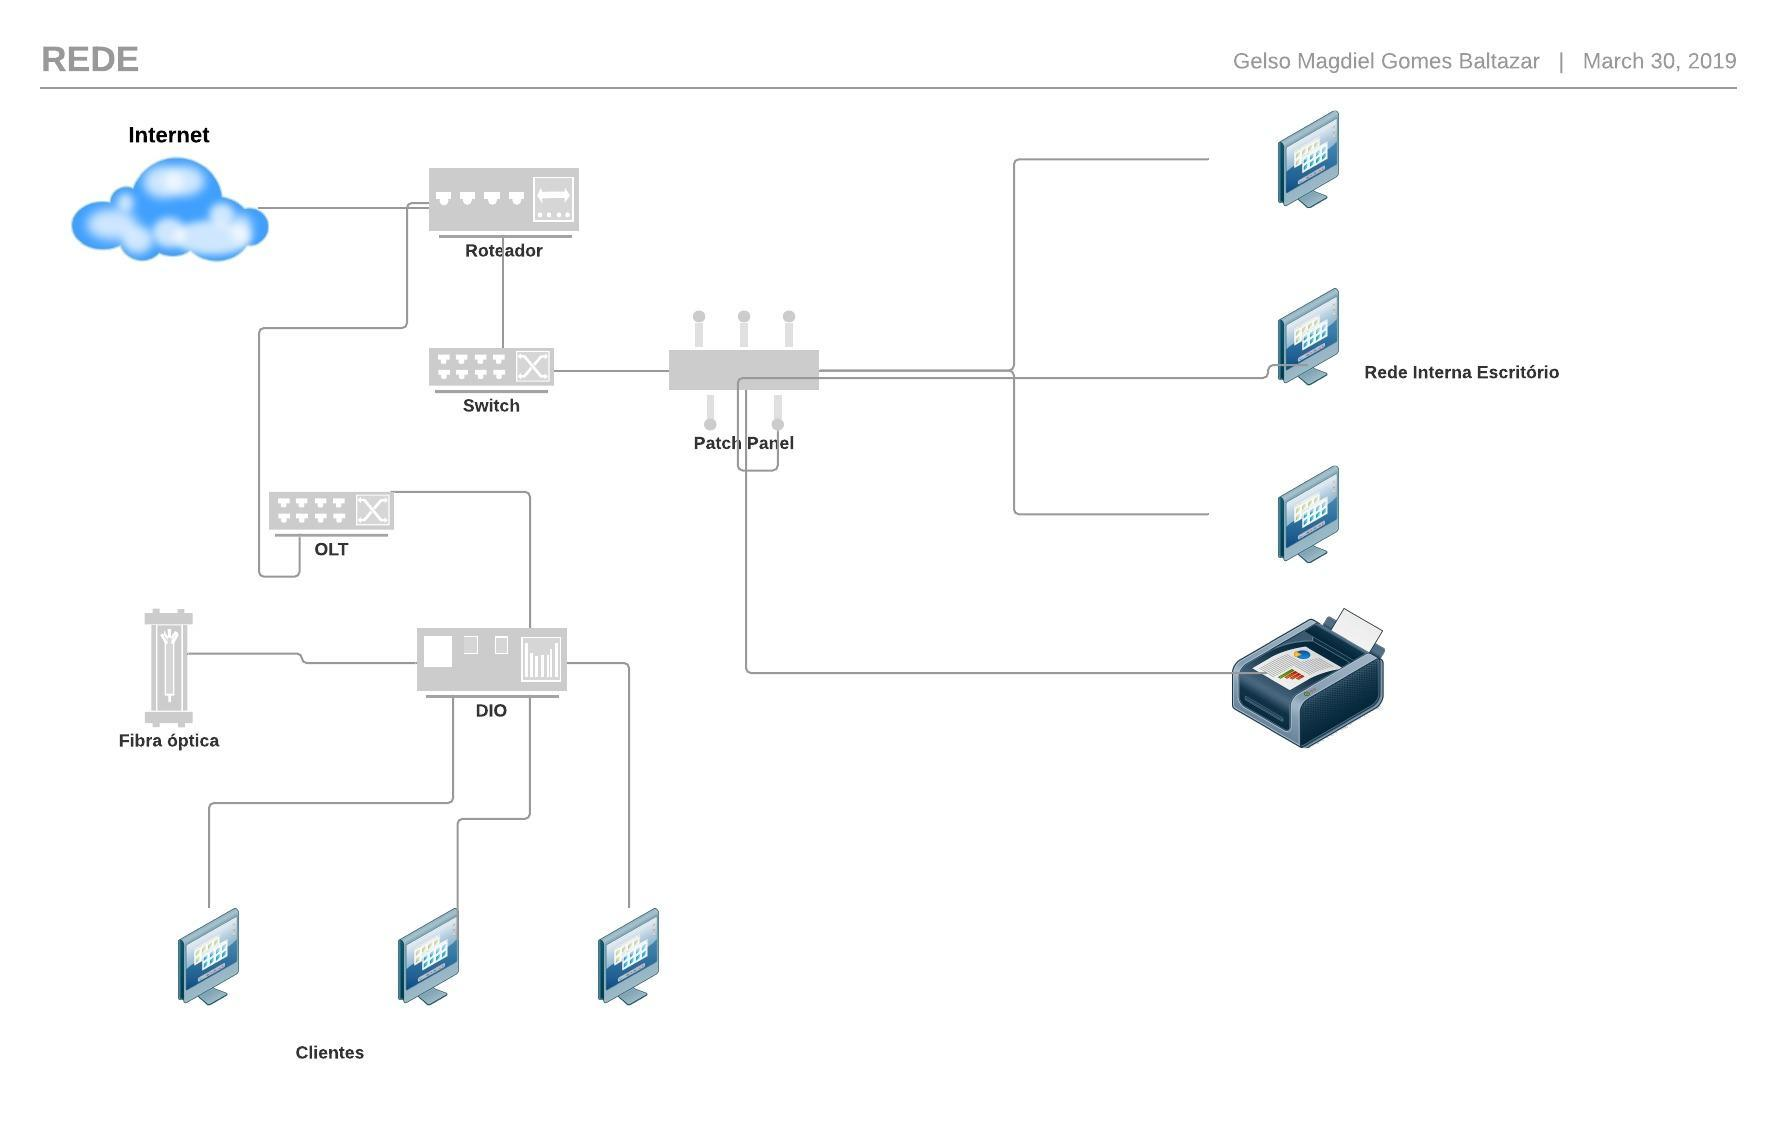
\includegraphics[width=\textwidth]{topologia}
		\caption{Topologia da rede}
		\label{topologia}
	\end{figure}
	
	
	\subsection{Memorial descritivo}
	
	01 - Switch TP-Link TL-SG3424
	01 - Switch TP-Link TL-SG1024
	01 - Roteador Mikrotik CCR1016
	01 - OLT DATACOM DM4610
	01 - Patch Panel 24P Furukawa CAT6 Gigalan
	10 - Patch Cord CAT6 Furukawa
	01 - Patch Cord Óptico LC
	04 - Jack RJ45 CAT6 FURUKAWA
	
	\subsection{Identificação dos cabos}
	Os cabos serão identificados por numeração. Na parede onde está cada ponto de rede haverá um número, que deverá ser correspondente ao mesmo número no patch cord. Ex: Porta 1 do patch cord será o ponto 1 marcado na parede.
	Para interligação dos equipamentos no rack, os cabos serão numerados nas duas pontas.
	
	\section{Implantação}
	A implantação deverá ser executado de madrugada para não causar indisponibilidade de serviços aos clientes durante período comercial. O projeto deverá ser concluído em até 4 dias.
	Iniciando no dia 06/04/2019 a partir das 1:00 hr com término às 5:00. Conforme conograma abaixo:
	Dia 01 - Cabeamento óptico:
	\begin{itemize}
		\item Organização;
		\item Identificação;
		\item Troca de equipamentos que forem necessários;
		\item Certificação;
		\item Documentação;
	\end{itemize}
	Dia 02 - Cabeamento elétrico:
	\begin{itemize}
		\item Organização;
		\item Identificação;
		\item Troca de equipamentos que forem necessários;		
		\item Documentação;
	\end{itemize}
	Dia 03 - Configurações:
	\begin{itemize}
		\item Roteador;
		\item Switchs;	
		\item Documentação;
	\end{itemize}	
	
	\section{Plano de certificação}
	A certificação será realizada somente na rede óptica para identificar possíveis atenuações ou rompimentos. E a mesma deverá ser realizada no mesmo dia que em que serão ornigazados os cabos ópticos.
	
	\section{Plano de manutenção}
	
	Revisões deverão ser realizadas a cada 12 meses.
	
	\subsection{Plano de expansão}
	Em caso de necessidade de expansão da rede, há 19 portas vagas no switch para novas instalações.  Para essas possíveis instalações, serão necessários apenas instalar os Jack RJ45 na parede e conectá-los ao patch panel, e do patch panel conectar um patch cord até o switch.
	
	\section{Risco}
	\begin{itemize}
		\item Causar indisponibilidade do serviço após às 5:00;
		\item Quebrar cabos ópticos;
		\item Conectar cabos em portas errados;
	\end{itemize}	
	
	
	\section{Orçamento}
	Pelo fato de ser somente reorganização do rack, será cobrado valor de RS200,00 à hora de serviço, e equipamentos se forem necessários trocar. No valor mencionado está incluso a certificação.
	
	\section{Recomendações}
	É recomendado não realizar instalações ou manutenções sem o devido conhecimento. Para manutenções ou instalações é recomendado contratar técnicos especializados para que haja o melhor funcionamento da rede.

	
\end{document}